% Chapter Template

\chapter{Implementation} % Main chapter title

\label{Chapter4} % Change X to a consecutive number; for referencing this chapter elsewhere, use \ref{ChapterX}

\lhead{Chapter 4. \emph{Implementation}} % Change X to a consecutive number; this is for the header on each page - perhaps a shortened title

%----------------------------------------------------------------------------------------
%	SECTION 1
%----------------------------------------------------------------------------------------

\section{Introduction}

This chapter describes the implementation of an experiment undertaken to answer the research question proposed by this thesis. A critical first step in performing that experiment is the implementation of a defeasible reasoning system. This is taken as a starting point for this chapter. 

The application architecture and programming decisions that were made are explained and justified with respect to how they support the experiment. The challenges associated with implementing a system of this nature are presented along with the solutions pursued to overcome those challenges.

The implementation of the experiment is then discussed. Specific details of how events unfolded are mentioned where they are relevant to discussion in the evaluation section.

\section{Defeasible Reasoning Software Implementation}

The research question of this dissertation deals specifically with an implementation of defeasible reasoning. The design of the system was outlined in chapter ~\ref{Chapter3} without any specific implementation details discussed. 

It was decided to implement the software as a web application. In the last 10 years web browser technology has improved vastly. Advances such as HTML5 APIs, powerful Javascript engines and mobile technology allows fully featured applications to be developed and run in the browser. 

Developing the application as a web based one offers a number of practical advantages to the experiment. Participants in the experiment can access the application remotely from anywhere. The software is platform independent and can run on any web browser with Javascript enabled. No software needs to be installed on different machines. No software needs to be updated locally, just once on the application server. All of the data associated with the DR experiment is all located and stored on the server allowing it to be retrieved easily for analysis.

%-----------------------------------
%	SYSTEM ARCHITECTURE
%-----------------------------------
\subsection{System Architecture}

In chapter~\ref{Chapter3} the required system functionality was designed and relevant components identified. The functionality of eliciting the knowledge base (the AF and membership functions) and the verification of this knowledge base is implemented as a Javascript client application. This communicates with a back-end server that provides a RESTful Web service written in PHP (using the Slim Framework\footnote{\url{www.slimframework.com}}).

The Web Service back-end provides the basic functions outlined for the application. The back-end saves a knowledge base to disk as a JSON file. The Javascript client can request a  list of knowledge bases and from this list retrieve a knowledge base previously created by the user. Knowledge bases were saved as JSON files on disk rather than in a database. This allowed structure of the application to change more fluently during development. It also supports knowledge bases to be examined and serialized in their complete form without needing to assemble it with queries from the database. The server allows the client to access data stored as CSV files so that an expert can evaluate their knowledge base against the data. 
The last critical component of the server application is to take a row from the data set and compute the value of the construct using the knowledge-base.

The application is served from an apache server running on a virualised Ubuntu instance provided by the Okeanos project \footnote{\url{okeanos-global.grnet.gr}}.

In order to speed up the development process a number of open source frameworks and libraries have been utilised in the software implementation. The CSS framework Bootstrap\footnote{\url{getbootstrap.com}} and the Javascript library JQuery\footnote{\url{jquery.com}} have been used for presentational aspects of the site. Bootstrap provides a number of useful components such as modal boxes tjat allow the software to present information to the user in a clear manner. JQuery provides wrappers arround native browser functionality such as DOM manipulation and AJAX networking facilities that abstract away the inconsistencies between browser implementations.

The graphical input of argumentation frameworks and membership functions is achieved using the  D3 library\footnote{\url{d3js.org}} developed by Bostock et al.\cite{2011-d3} D3.js is a data visualisation library that allows developers and designers to interact with data in the browser. Data can be loaded from urls in multiple formats such as JSON and CSV. Data points can be ``attached'' to DOM elements which provides useful functions. The styling of the DOM element can be linked to the value of the data and the data can be manipulated by user interactions. D3 is most commonly used with SVG\footnote{\url{www.w3.org/Graphics/SVG/}} (Scalable Vector Graphics) a markup language for implementing vector graphics. SVG has been an open standard for more than 10 years now, as a result it has been widely implemented and there is currently more support for it than other graphics alternatives such as HTML5 Canvas. Two key features of D3 that are used in the implementation of the experiment software are its implementation of Bezier curves and its force directed graph implementation.

The server implementation requires Argumentation semantics to be computed based on the input of a Dung Argumentation Framework. Computing these semantics efficiently requires a deep understanding of argumentation theory, graph theory and algorithms. This implementation is specialised and a number of libraries have been explored in the literature review for its implementation. Dung-o-matic, an implementation of these algorithms has been made available by the University of Dundee under the Apache License, Version 2.0. The Dung-o-matic\footnote{\url{www.arg-tech.org/index.php/projects/dung-o-matic/}} was found not to be the most efficient implementation for the computation of semantics by a number of studies (see \ref{sec:dr_implementations}). However, its source code is freely available and can be run on any platform provided the platform has Java installed. Moreover, the advantage of using Java is that as one of the world's most popular programming languages there is abundant documentation available to assist in its integration. The source code for both dynPARTIX and ConArg2 are unavailable and cannot be used for implementation in this project. It could be possible to integrate ASPARTIX for a more efficient implementation, however, this requires an answer set programming solver to be installed. It is anticipated that the integration of such a solver could be laborious and time consuming without adding much value to the project. For these reasons the Dung-o-matic was chosen despite performance concerns.

The technologies outlined in this section are manifested in the application architecture in figure~\ref{fig:AppArch}. With these underlying technologies established a number of implementation challenges remain. The solutions to these challenges are the focus of the following chapters.

\begin{figure}[h]
    \centering
    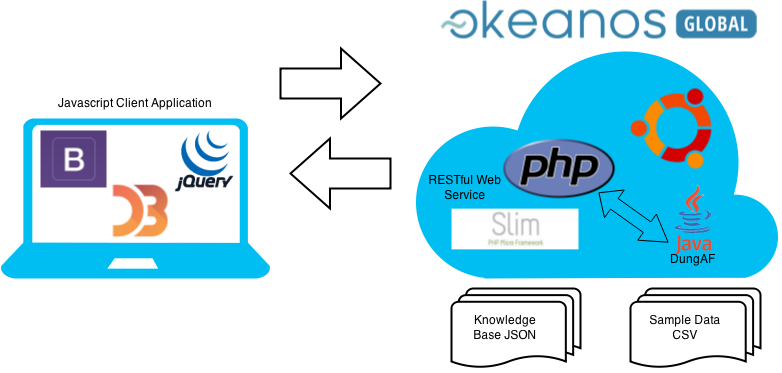
\includegraphics[width=1\textwidth]{apparchitecture}
    \caption{Application Architecture}
    \label{fig:AppArch}
\end{figure}

%-----------------------------------
%	SYSTEM ARCHITECTURE
%-----------------------------------
\subsection{Application Front End}

The two crucial features of the application front-end are the interface for drawing argumentation frameworks and the interface for drawing membership functions. The implementation of these features is discussed here.

The implementation leverages D3's force-directed layout\footnote{\url{https://github.com/mbostock/d3/wiki/Force-Layout}}, a built in layout that solves the problems posed when visualising graph data structures. Typical data visualisation techniques take values and parse them one by one, drawing a marker in a position based on each value. This is not the case with graph data structures. With graph data structures, it is generally preferable to have vertices that have common edges close together and to have those without common edges far apart. D3's force directed layout takes list of vertices and edges and generates positions for vertices using simulation inspired by physics. Similarly to sub-atomic particles, nodes are given charges that repel other nodes in the graph and are kept from drifting apart by the links in the graph. There is also a force at the center of the visualisation that prevents any of the nodes from drifting outside the view port. 

By utilising this layout and D3's event helpers (listeners for mouse actions such as click and drag) an interface can be implemented that allows a user to input a directed graph, or in the case of the experiment, an argumentation framework. The user can create a node by clicking on an empty space on the graph and can create links between two nodes by dragging from one node to another. When the user creates a node they are prompted to give the node a label. This results in a knowledge base being represented as in listing~\ref{lst:kbds}.


\begin{lstlisting}[caption={JSON data structure for argumentation framework},label={lst:kbds}]
knowledge_base {
  nodes : [
    {
      id: 0
    },
    {
      id: 1
    },
    {
      id: 2
    }
  ],
    lastNodeId : 2,
    links : [
      {source: nodes[0], target: nodes[1], left: false, right: true },
      {source: nodes[1], target: nodes[2], left: false, right: true }
  ]
}
\end{lstlisting}

D3 expects the data as an array of node objects and an array of links which contain references to the nodes. It adds x and y values to the nodes to track their position in the viewport and updates theses values at a fixed interval in order to animate the graph. The id of the last node added to the viewport is stored in the \lstinline{lastNodeId} variable. This is important for creating new nodes as nodes are tracked based on their IDs, not their array indexes. 

Three types of attack relation must be modeled by the interface for correct implementation of the system. These attacks are undercutting attacks, rebutting attacks and mitigating arguments. Undercutting attacks are implemented simply as an arrow from the attacking node to the attacked node. In the data structure this is modeled as a link with the value for either `right' or `left' equal to true. In a rebuttal attack both arguments attack each other. This link is visualised as an arrow with two ends. In the data structure this is represented by setting both `right' and `left' equal to true. Examples of these arguments visualised using the tool are shown in figure~\ref{fig:undercutting} and figure~\ref{fig:rebuttal}. Mitigating arguments are modeled the same as undercutting arguments but are represented in the system by labeling their output functions as ``mitigating arguments''.

\begin{figure}
\subfloat[An undercutting attack\label{fig:undercutting}]
  {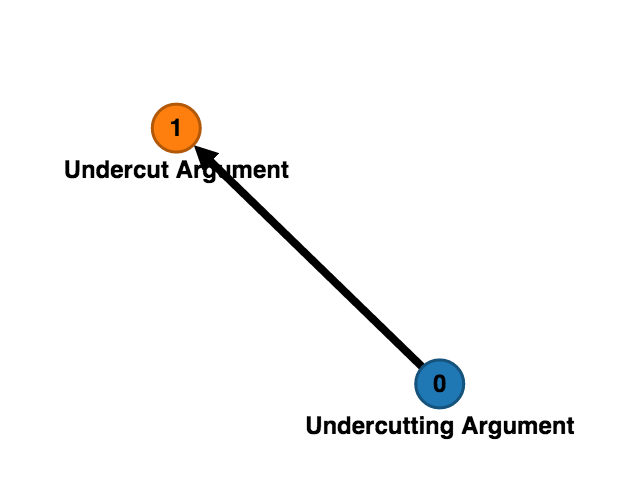
\includegraphics[width=.49\linewidth]{undercutting}}\hfill
\subfloat[A rebuttal attack\label{fig:rebuttal}]
  {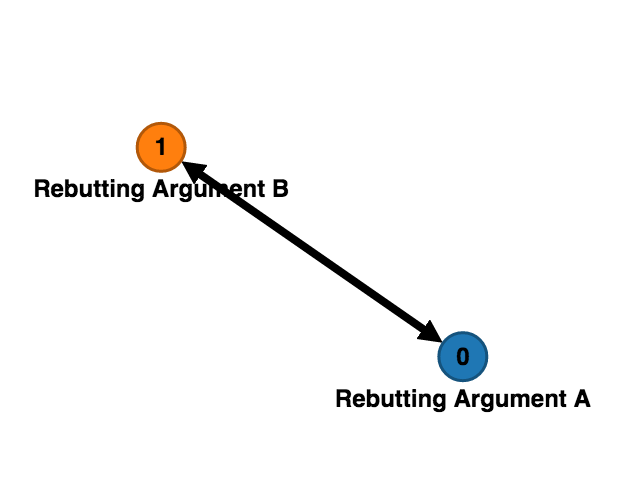
\includegraphics[width=.49\linewidth]{rebuttal}}\hfill
\caption{Examples of different attacks drawn using the interface}
\end{figure}

By selecting a node in the graph a user can then define membership functions representing the internal premises of the argument and an output function representing the contribution of the truth of this argument to the overall value of the construct. It was decided in the system design phase that the user should be able to draw these functions using the interface. It was decided to utilise Bezier curves to achieve this in a manner that is simple to implement, usable and that would facitiate easy representation, storage and serialisation of membership functions. 

According to \cite{farin2002handbook}, Bezier curves provide a ``geometric-based method for describing and manipulating polynomial curves and surfaces.'' Bezier curves are parametric curves in which each point on the curve is a function of the parameter \textit{t}. Bezier curves are defined by a number of control point that they interpolate. The curves begin at their first control point x(0) and end at their last control point x(1).

Bezier curves may be defined recursively is draw on for their implementation in the system. Given a Bezier curve $\mathbf{B}_{\mathbf{P}_0\mathbf{P}_1\ldots\mathbf{P}_n}$ with points $\mathbf{P}_0\mathbf{P}_1\ldots\mathbf{P}_n$ the recursive definition of a curve is:

\begin{equation}
\label{math:recursivedef}
$$
\mathbf{B}(t) = \mathbf{B}_{\mathbf{P}_0\mathbf{P}_1\ldots\mathbf{P}_n}(t)
= (1-t)\mathbf{B}_{\mathbf{P}_0\mathbf{P}_1\ldots\mathbf{P}_{n-1}}(t) + t\mathbf{B}_{\mathbf{P}_1\mathbf{P}_2\ldots\mathbf{P}_n}(t)
$$
\end{equation}

where $\mathbf{B}_{\mathbf{P}_0}(t) = \mathbf{P}_0}$ and $\mathbf{B}_{\mathbf{P}_n}(t) = \mathbf{P}_n}$.

D3 provides methods for manipulating SVG, which defines its `paths' (Bezier curves) using control points. By providing the user with a collection of control point the can drag it is possible for them to define curves however they please. It also provides the advantage of allowing membership functions and output functions to be  defined simply as control points in the data model. As bezier curves exist within the range 0 and 1 on the x and y axis the associated values must be scaled to the users desires. Users can input minimum and maximum values that are used to scale the graph. These are stored with the membership function in the JSON data structure for later processing. From this a single argument can be defined in JSON as in listing~\ref{lst:arg_memfunc}. In order to allow users to create membership functions quickly functionality was implemented to allow the user to save previously used functions as template functions as can be seen in figure~\ref{fig:membfunc}.

\begin{figure}[!h]
\label{fig:membfunc}
\centering
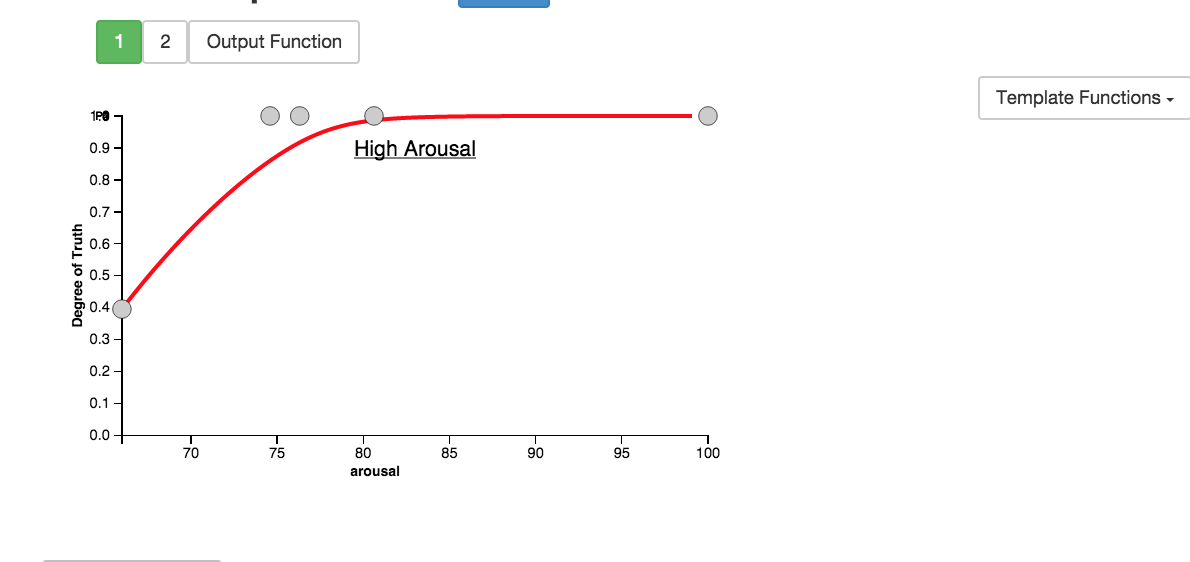
\includegraphics[width=1\textwidth]{membershipfunction}
\caption{An interface that allows a user to `draw' a membership function using Bezier curves}
\end{figure}


\begin{lstlisting}[caption={JSON data structure a node including its fuzzy membership functions},label={lst:arg_memfunc}]
    {
      id: 0,
      "name": "MD1",
      membership_functions: [{
      title: "Low Effort->Low MWL",
      points: [{x: 1, y: 25}, {x: 0, y: 0}, {x: 10, y: 0}, 
                {x: 20, y: 25}, {x: 22, y: 12}],
      xLabel: "Effort",
      yLabel: "Degree of Truth",
      xMin: 0,
      xMax: 50,
      yMin: 0,
      yMax: 50,
    },
    {
      title: "Low Performance->High MWL",
      points: [{x: 10, y: 140}, {x: 30, y: 0}, {x: 140, y: 0},
                {x: 200, y: 150}, {x: 125, y: 125}],
      xLabel: "Performance",
      yLabel: "Degree of Truth",
      xMin: 0,
      xMax: 250,
      yMin: 0,
      yMax: 300,
    }
    ],
    "output_function": {
        "title": "Underload",
        "xLabel": "Degree of Truth",
        "yLabel": "Mental Workload",
        "xMin": 0,
        "xMax": 1,
        "yMin": 0,
        "yMax": 33,
        "points": [
          {"x": 0.00454,"y": 33},{"x": 0.222,"y": 24.849},
          {"x": 0.46136,"y": 16.954},{"x": 0.65681,"y": 10.3458},{"x": 1,"y": 0}]
      },
    }
\end{lstlisting}

There is a flaw in this approach that should be noted. In order to compute the users beliefs accurately the membership function should follow the strict mathematical definition of a function; that it should only output a single value for any input. Bezier curves do not obey this rule as they are parametrised by \textit{t} and as a result it is possible for users to draw functions like in figure~\ref{fig:badness}. It is also possible for users to define functions with no corresponding output for a given figure. If a user does the system will compute an incorrect value for the premise and the result will be compromised. Participants in the experiment are made aware of this before undertaking the experiment.

\begin{figure}[h]
\label{fig:badness}
  {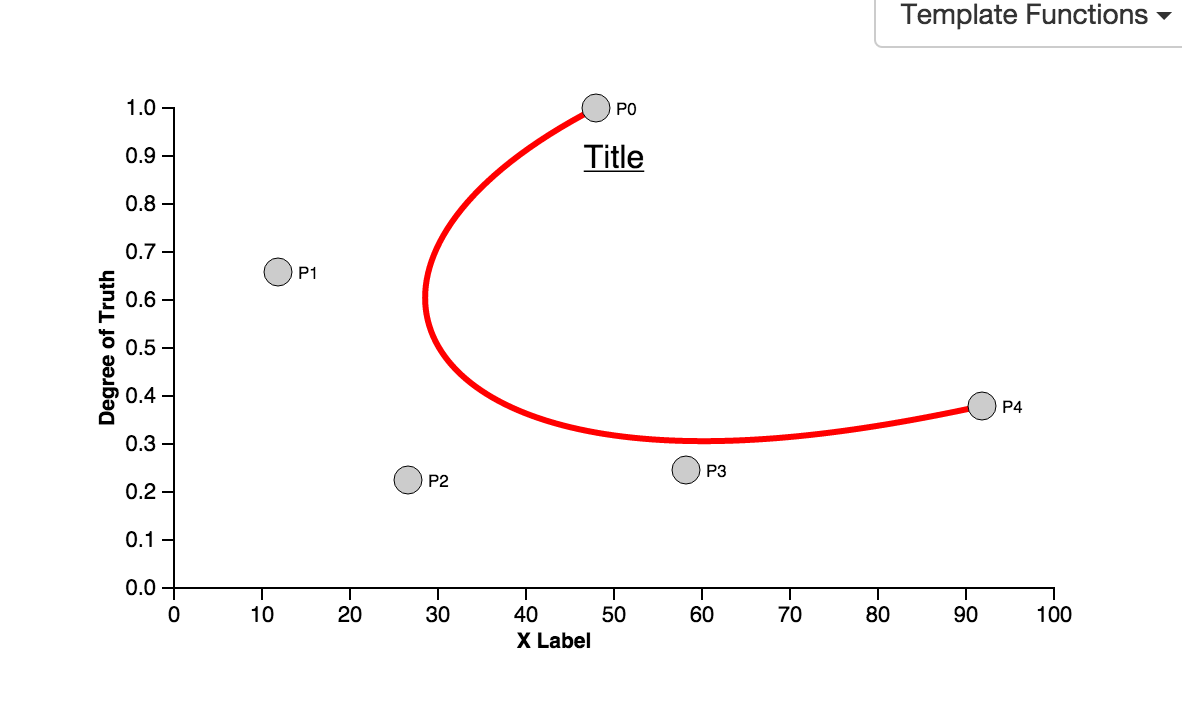
\includegraphics[width=.3\linewidth]{badness1}}\hfill
  {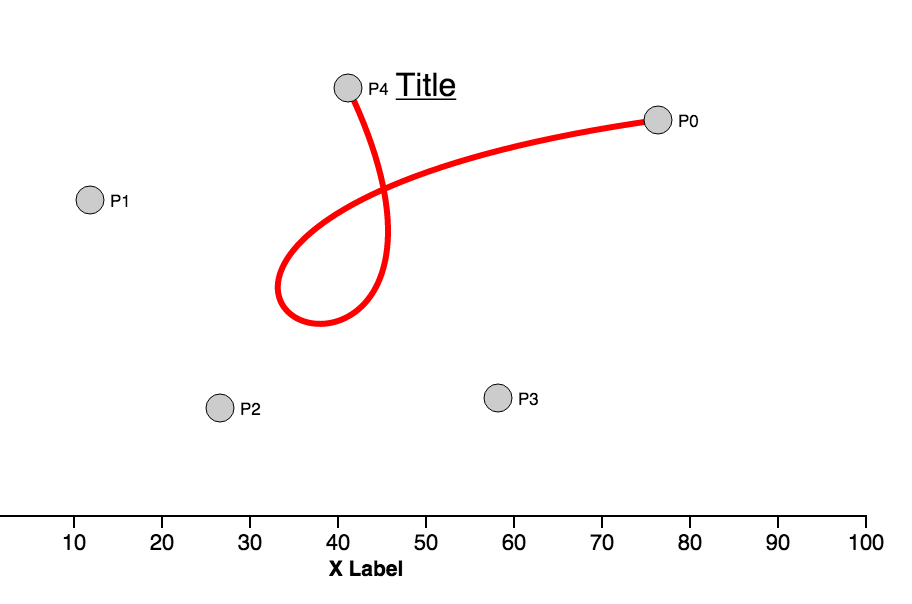
\includegraphics[width=.3\linewidth]{badness2}}\hfill
  {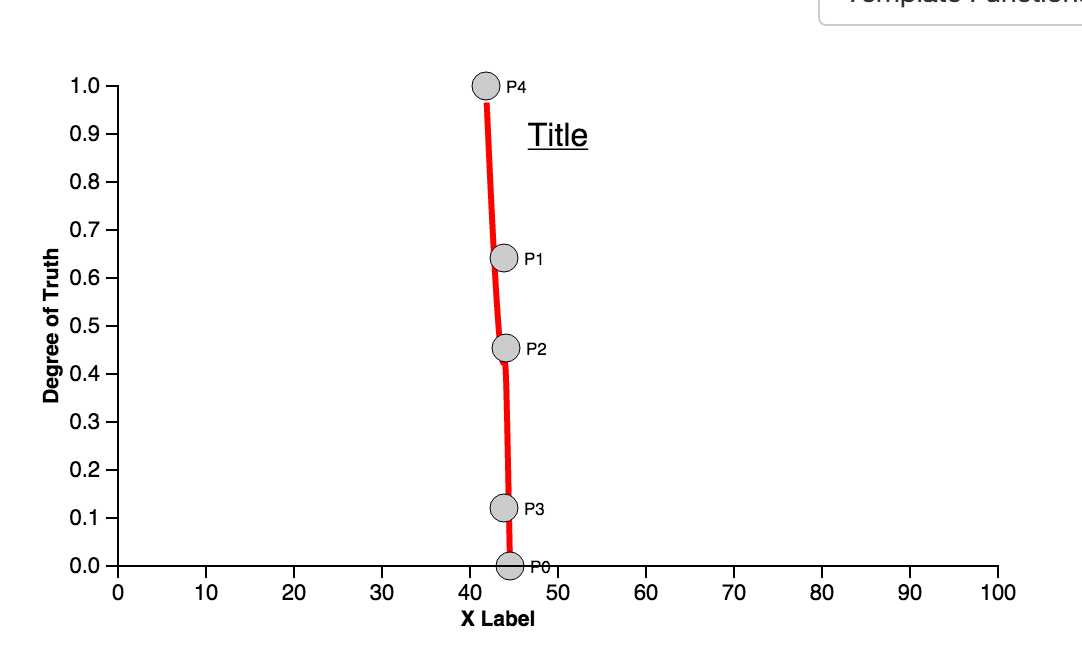
\includegraphics[width=.3\linewidth]{badness3}}\hfill
\caption{Examples of Bezier curves that can be drawn that are not functions}
\end{figure}

With the argumentation framework and membership function finally implemented the web interface appears as in figure~\ref{fig:finalUI}.

\begin{figure}[!h]
\label{fig:finalUI}
\centering
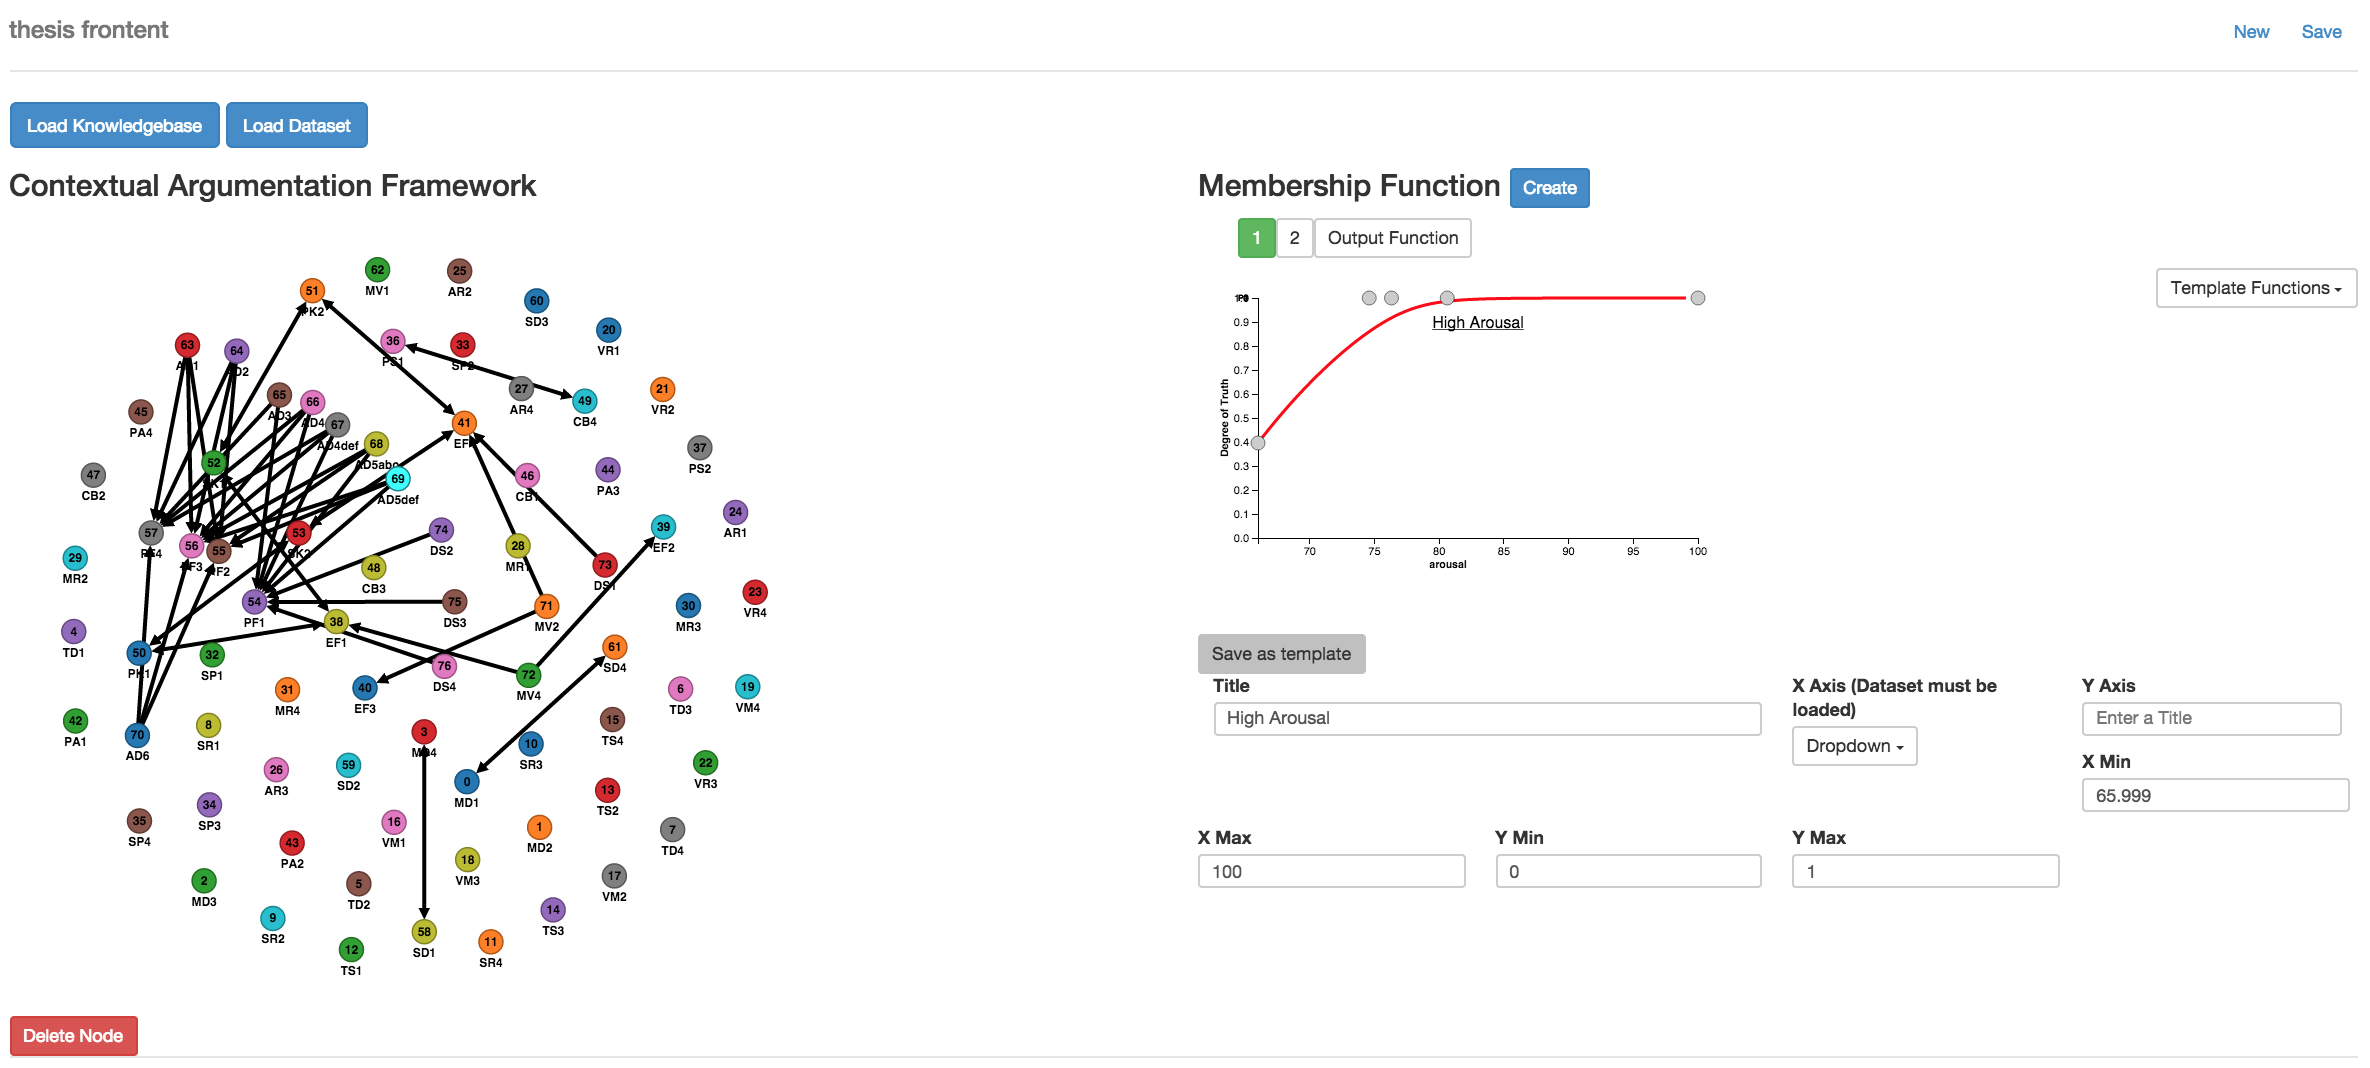
\includegraphics[width=1\textwidth]{Fullscreen}
\caption{The fully developed tool for eliciting knowledge bases}
\end{figure}

Once a knowledge base has been elicited from a user they can test their with the system by computing results. They can download a sample data set which is displayed as in figure~\cite{fig:sampleData}.

\begin{figure}[!h]
\label{fig:sampleData}
\centering
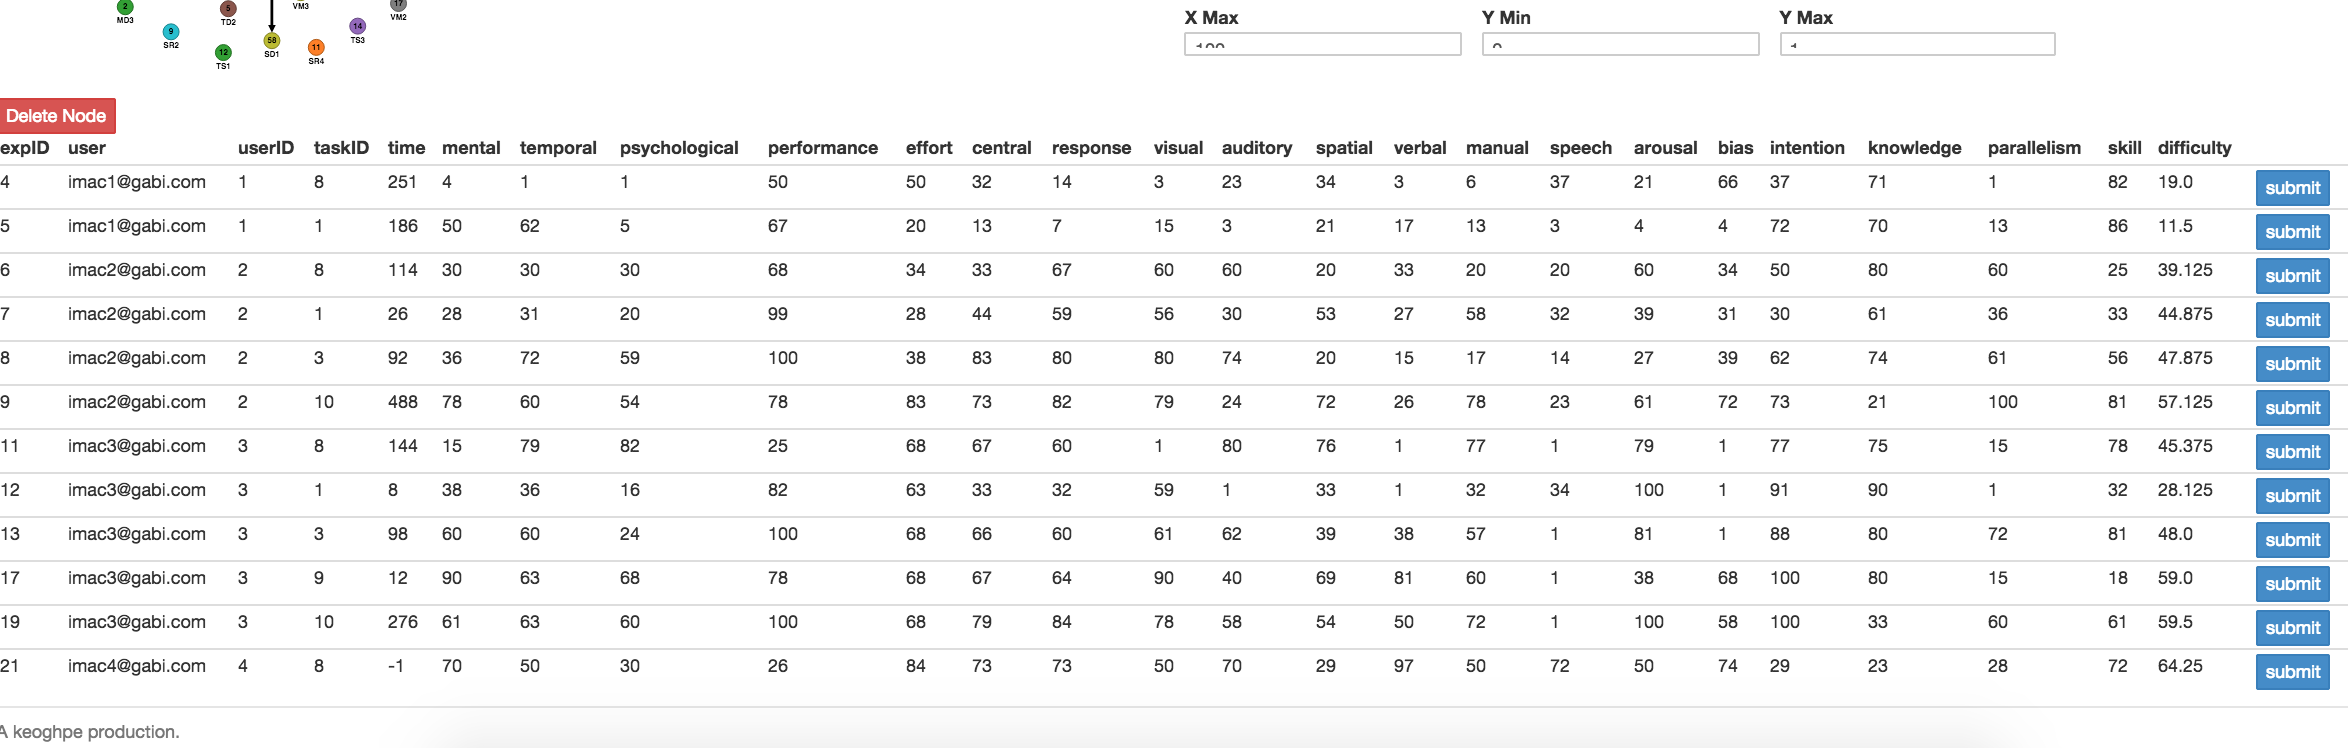
\includegraphics[width=1\textwidth]{data}
\caption{A selection of data for the user to test their knowledge base with}
\end{figure}

For a single row in the data the user can choose from a selection of semantics to run on the data (see figure~\cite{fig:semantics}).

\begin{figure}[!h]
\label{fig:semantics}
\centering
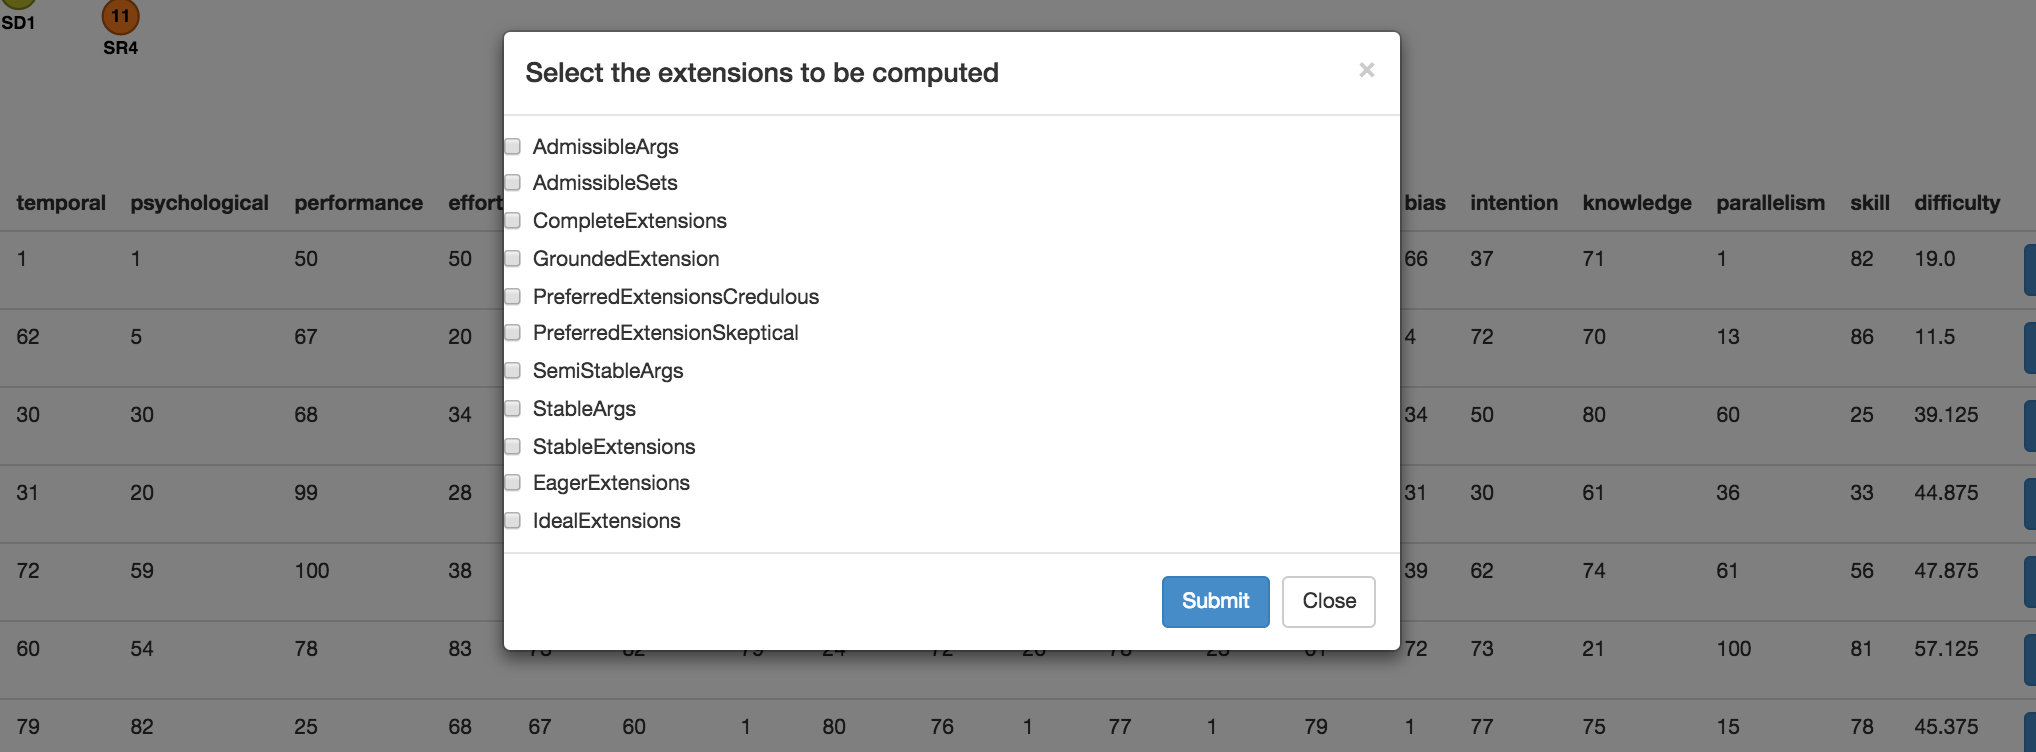
\includegraphics[width=1\textwidth]{options}
\caption{A list of options for semantics that can be computed by the system}
\end{figure}

The results of running the semantics are then presented to the user in the form given in figure~\cite{fig:semantics_results}. The results present an overall value for the construct as well as the total degree of truth of the semantic. Each argument that contribute to the semantic is returned as well as a degree of truth value and the value of the construct computed for that value. This extra information allows the user to scrutinise their knowledge base and its associated results further.

\begin{figure}[!h]
\label{fig:semantics_results}
\centering
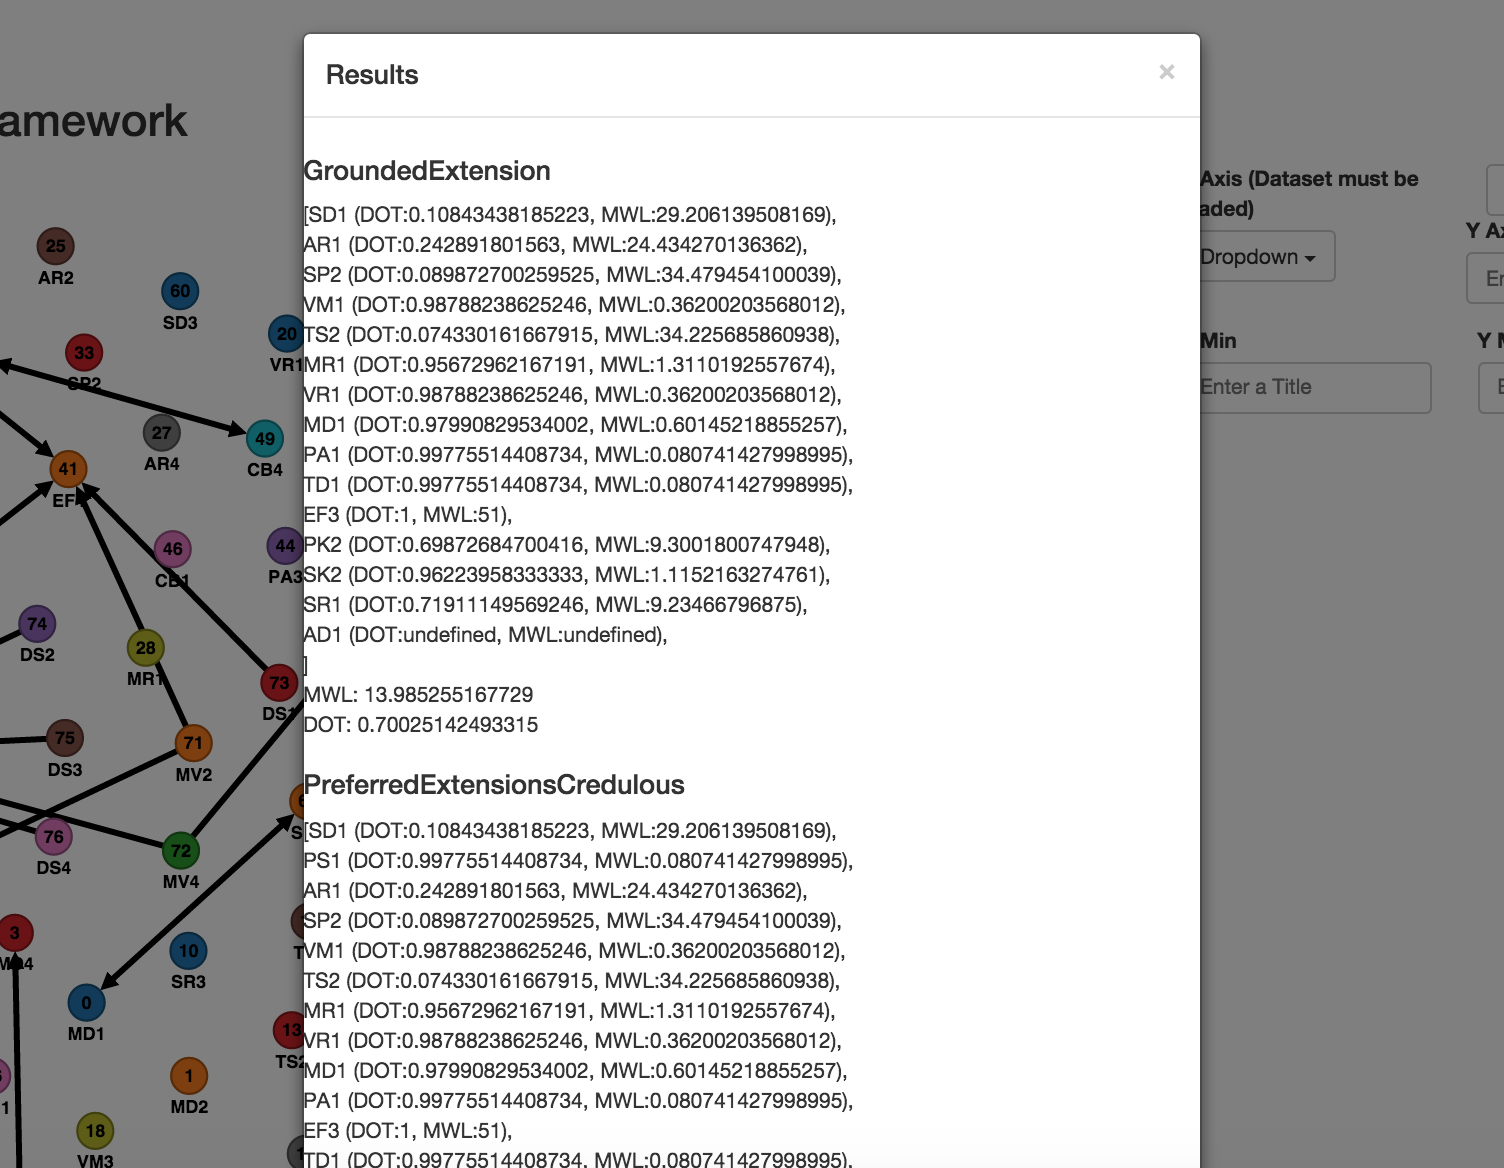
\includegraphics[width=1\textwidth]{results}
\caption{Results of computing the semantics on the framework. (Undefined values belong to mitigating arguments)}
\end{figure}

\subsection{Application Back-End Implementation}

The application back-end implements a REST architecture that allows the front-end to retrieve data via AJAX requests. A summary of the REST API is outlined in table~\ref{tab:rest_routes}.

\begin{table}[]
\centering
\begin{tabular}{|l|l|L{5cm}|}
 URL & Request Method & Functionality \hline \\
 \lstinline{/} & POST & Compute the Knowledge Base result for a given row of data
 \lstinline{/knowledgebases/} & GET & Return a list of Knowledge Bases saved on the server
 \lstinline{/knowledgebases/:filename} & GET & Retrieve a specific knowledge base named \lstinline{:filename}
 \lstinline{/knowledgebases/:filename} & POST & Save a knowledge base in a JSON file named \lstinline{:filename}
 \lstinline{/datasets/} & GET & Return a list of data sets saved on the server
 \lstinline{/datasets/:filename} & GET & Retrieve a specific data set csv file named \lstinline{:filename}
\end{tabular}
\caption{Caption}
\label{tab:rest_routes}
\end{table}

In order to compute the result for a single row in the data set the front end sends a POST request containing the knowledge base nodes and links, the row in the data and a list of semantics to be computed. A PHP class \lstinline{FrameworkRunner} copies these values into a local list of arguments and attacks.

The first step in the process is to determine which arguments are activated. This is done by looking at each argument and determining if each of its premises are satisfied by the data in the row. For an individual premise the value of data associate with its x label is retrieved. If this value is between the premise's \lstinline{xMin} and \lstinline{xMax} values then the premise is relevant. If the value falls outside these bounds then the parent argument and its associated attack relations are discarded. 

The sub-graph of activated arguments and their attack relations remains in the class to compute semantics for. In order to compute the semantics the Dung-o-matic Java class is wrapped in another class that allows it to read a list of arguments and attacks as a string and return the results in a similar format. The \lstinline{FrameworkRunner} class produces a string containing the IDs of the nodes in the format expected by this Java class. The Java class has been exported as an executable JAR file which is then called from PHP using the \lstinline{exec()} function and passing this simple string as an argument. The Java code returns JSON object with the name of the computed semantic as keys and the sub-graphs as an array of arrays associated with those keys.

Once the semantics have been computed for an Argumentation Framework the values associated with each argument can be computed. For a given row in the data set, the results for an argument remain the same no mater what the configuration of the framework is. This allows us to cache the output value of an argument in memory rather than having to recompute the same values for each semantic. The results are computed on the server using a Bezier curve implementation. 

The Bezier curve computation is implemented in a PHP class \lstinline{Bezier}. This class contains methods to compute the X and Y values for a point on the line given a list of control points and a value for \textit{t}. It provides two other methods \lstinline{yFromX} and \lstinline{xFromY} that compute a value for Y given X and vice versa. The Bezier curve implementation is based on the recursive definition given in equation~\ref{math:recursivedef}. its implementation is given in Algorithm~\ref{alg:recursive}.

\begin{algorithm}[H]
\label{alg:recursive}
\SetAlgoLined
\KwData{A list of control points $L = \mathbf{P}_0\mathbf{P}_1\ldots\mathbf{P}_n$ and a value $t$}
\KwResult{A point $P = (X,Y)$ corresponding to \textit{t}}
  \SetKwFunction{bezier}{bezier}
  \SetKwProg{myalg}{Algorithm}{}{}
  \myalg{\bezier{$L$, \textit{t}}}{
    \eIf{there is only one control point in $L$}{
        \KwRet $\mathbf{P}_0$\;
        }{
        
        $\mathbf{P}_0 \leftarrow$ \bezier{$\mathbf{P}_0\mathbf{P}_1\ldots\mathbf{P}_n-1$,  \textit{t} }
        
        $\mathbf{P}_1 \leftarrow$ \bezier{$\mathbf{P}_1\mathbf{P}_2\ldots\mathbf{P}_n$,  \textit{t} }
        
        $X \leftarrow (1 - t)\mathbf{P}_0_X + t\mathbf{P}_1_X $
        
        $Y \leftarrow (1 - t)\mathbf{P}_0_Y + t\mathbf{P}_1_Y $
        
        \KwRet $(X, Y)$\;}{}
        }
\caption{Computing a point on the curve for a given value of \textit{t}}
\end{algorithm}

For a given membership function with fixed values for its control points any point on the curve can be described by a value t between 0 and 1. By passing t into the function we obtain a value for x and y. As it is not possible to simply pass in an x value and obtain a corresponding y value we must search for y by varying the parameter t. This is done efficiently using a binary search algorithm. For each iteration we pass in two values of t to get two values of x and compare them with our target x value. We continue to search a space closer and smaller to x until we arrive at a value that is within a threshold we consider to be satisfactory. From this point we can obtain the Y value. The pseudocode for this algorithm is given in Algorithm~\ref{alg:bin_search}.

\begin{algorithm}[H]
\SetAlgoLined
\KwData{A list of control points $L = \mathbf{P}_0\mathbf{P}_1\ldots\mathbf{P}_n$, a tolerance $T$ and a value $X$}
\KwResult{A value for $Y$ corresponding to the input $X$}
\SetKwFunction{bezier}{bezier}

$t_{lower} \leftarrow 0$

$t_{upper} \leftarrow 1$

\While{The computed $X$ values are outside the tolerance $T$ of $X$}{
  
  $P_{lower} \leftarrow$\bezier{$L$, $t_{lower}$}
  
  $P_{upper} \leftarrow$\bezier{$L$, $t_{upper}$}
  
  \eIf{$P_{lower X}$ is closer to $X$ than $P_{upper X}$}{
  $t_{upper} \leftarrow t_{upper} + t_{lower} $
   }{
  $t_{lower} \leftarrow t_{upper} + t_{lower} $
  }
 }
\caption{Obtaining a value for $Y$ given an $X$ value}
\label{alg:bin_search}
\end{algorithm}

This calculation is performed for each membership function in the node and an average of the values of the output is produced. This corresponds to the overall degree of truth for the argument. This value is then used as the input to the output function which computes an overall construct value for that argument. If the output function of an argument is labeled as a mitigating argument then that argument is ignored.

Once the all of the argument construct values and degrees of truth are taken the overall results for the semantic can be computed. An overall construct value and degree of truth for the semantic is computed by taking the average of these values for each argument in the semantic. The client presents this information to the user in the evaluation interface previously presented.

The software was manually validated in order to determine that it was functioning correctly. Initially simple test cases were developed using the ASPARTIX online interface\footnote{\url{http://rull.dbai.tuwien.ac.at:8080/ASPARTIX/index.faces}} in order to validate that the argument evaluation was working correctly. Once the interface was working for small test cases it was evaluated by hand using an existing knowledge base. A number of bugs were discovered and fixed at this stage. The process continued iteratively until the implementation was considered to be of a quality appropriate to the experiment.

% Semantic algorithms

%-----------------------------------
%	EXPERIMENT IMPLEMENTATION
%-----------------------------------
\section{Experiment Implementation}

In order two provide a comparison of the ability of the defeasible approach to model a construct the knowledge bases of both an expert and a lay person were modeled using the tool developed in this chapter. The two knowledge bases provide a contrasting result and it is expected that the knowledge base of the expert will perform better than that of the lay person. These knowledge bases were saved on the server and evaluated in order to determine that they matched the expert's expectations.

\begin{figure}[H]
\centering
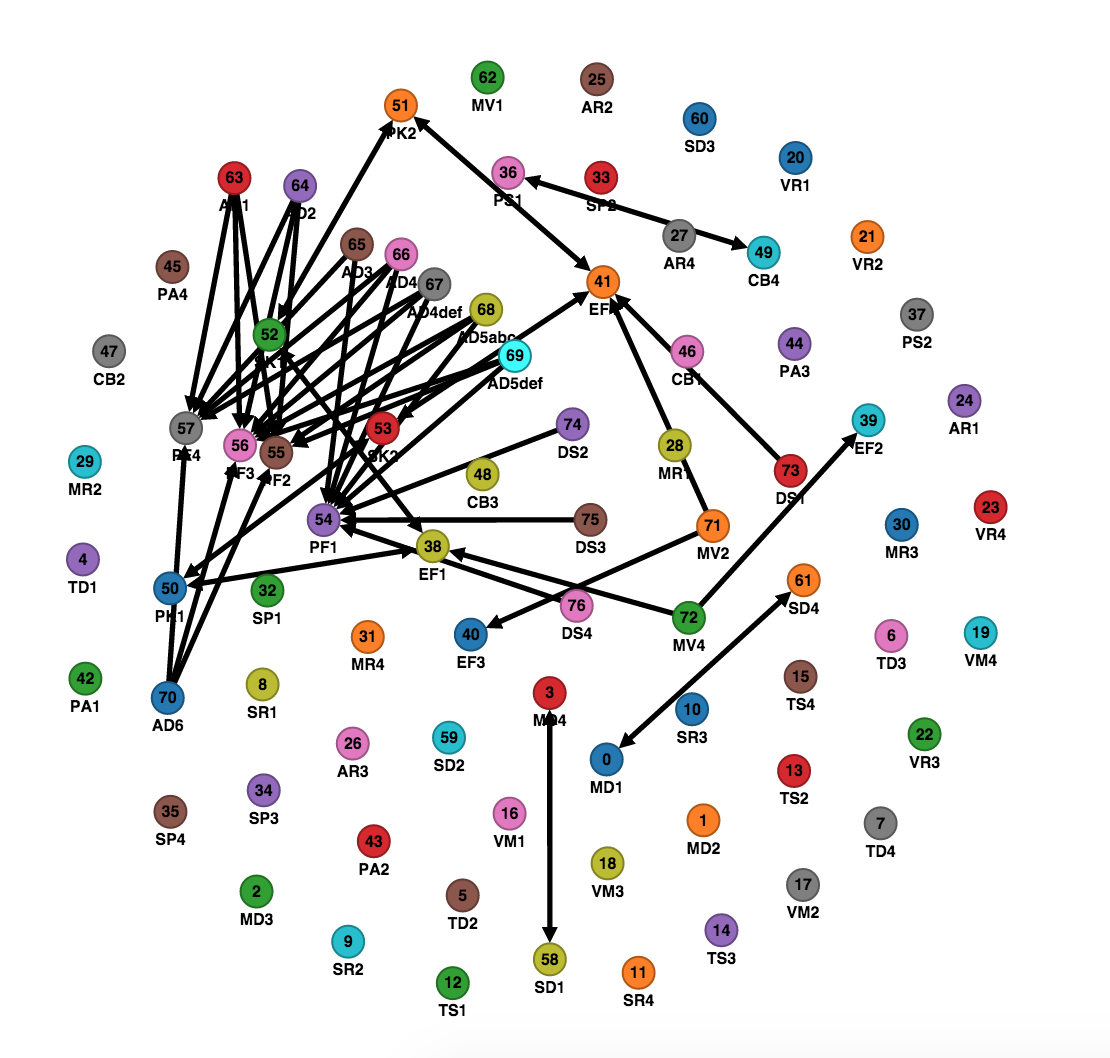
\includegraphics[width=1\textwidth]{ExpertAF}
\caption{The Argumentation Framework developed by the expert using the tool}
\end{figure}


As computing the semantics for an AF is an NP complete problem computing the results for a whole data set carries a large overhead for time. The time is considerably larger than the time of a typical HTTP request-response cycle so it was not feasible to compute all of the results for the data set in the web application format. 

In order to generate the results of running a knowledge base on a whole data set the \lstinline{FrameworkRunner} tool was wrapped in a command line tool written in PHP. Results were computed for the `grounded' and `preferred' extensions of the argumentation frameworks. The overall values for MWL for the extensions were collected for each row in the data. The time taken to compute these results was also collected in order to have an objective measure of the performance of the technique.

The second part of the research question was then answered by running machine learning algorithms on the experiment data using Weka. In order to assess regression algorithms task time was chosen as the dependant variable. Classification algorithms were testing using task ID as the dependent variable.

The regression algorithms used were additive regression, k-star, linear regression, multilayer perceptron, regression by simple linear regression and additive regression. These results were collected for each regression algorithm: correlation coefficient, mean absolute error, root means squared error, relative absolute error and root relative squared error.

In order to run classification algorithms on data, Weka requires the dependent variable to be in a string format. A simple python script was written to create a new column in the data set that would have the task numbers represented as letters $(1 \leftarrow A, 2 \leftarrow B, \ldots)$.
The classification algorithms used were bayes net, decision table, logistic regression, naive bayes and multilayer perceptron. The following metrics for these algorithms were collected: percentage of correctly classified instances, percentage of incorrectly classified instances, Kappa statistic, mean absolute error, root mean squared error, relative absolute error and root relative squared error. Confusion Matrices and a breakdown of accuracy by class (including TP Rate, FP Rate, Precision, Recall, F-Measure and ROC Area) was also collected for each model.

In order to determine the concurrent validity of the defeasible MWL models two regressions needed to be run on each model. The first regression is a linear regression using the values for MWL against time. The second is a logistic regression using the values for MWL against task number. Lastly in order to determine the convergent validity of the MWL values the Pearson co-relation of the values with other measured of MWL was determined.

\section{Conclusions}

This chapter outlined the implementation of an experiment and software to answer the research question posed by this project. The process of realising a tool used to elicit and perform computations on a defeasible knowledge base was described. Additional steps that needed to be taken in order that the software could be used to answer the question were explained.

The chapter briefly discussed the implementation of an experiment using the software and the machine learning work-bench Weka. Finally, the collection of extra data to analyse the experiment results was briefly discussed. The analyses of the information that has been gathered is the subject of the next chapter.